
% This LaTeX was auto-generated from an M-file by MATLAB.
% To make changes, update the M-file and republish this document.

\documentclass{article}
\usepackage{graphicx}
\usepackage{color}

\sloppy
\definecolor{lightgray}{gray}{0.5}
\setlength{\parindent}{0pt}

\begin{document}

    
    
\subsection*{Contents}

\begin{itemize}
\setlength{\itemsep}{-1ex}
   \item 1 - Derive A\_18x18 and Htilde\_2x18
   \item 2 - Perform integration
   \item 3 - Compare Residules of Observed and Computed Range and Range Rate
\end{itemize}
\begin{verbatim}
%%%%%%%%%%%%%%%%%%%%%%%%%%%%%%%%%%%%%%%%%%%%%%%%%%%%%%%%%%%%%%%%%%%%%%%%
%
%
% Zach Dischner-10/21/2012
%
% ASEN 5070-Statistical Orbit Determination
%
% Homework 7
%
%
%%%%%%%%%%%%%%%%%%%%%%%%%%%%%%%%%%%%%%%%%%%%%%%%%%%%%%%%%%%%%%%%%%%%%%%%

clc;clear all;close all; format compact;format long g;tic
\end{verbatim}


\subsection*{1 - Derive A\_18x18 and Htilde\_2x18}

\begin{verbatim}
% [A,Htilde]= FindA_Htilde();
% fprintf('A and Htilde were found. Not shown since they are too big to glean any insight from')
\end{verbatim}


\subsection*{2 - Perform integration}

\begin{verbatim}
%---------------------------------------------
%Constants
tol = 1e-13;
uE  = 3.986004415e14;               % m^3/s^2
J2  = 0.00108248;                   % []
Cd  = 2;
theta_dot  = 7.29211585530066e-5;   % rad/s
%---------------------------------------------


%---------------------------------------------
%Initial Conditions
time    = [0:20:18340];

RV_Init         = [757700,5222607.0,4851500.0,2213.21,4678.34,-5371.30];
Station_Init    = [-5127510.0 , -3794160.0 , 0.0 ,...               %101
                    3860910.0  , 3238490.0  , 3898094.0 , ...       %337
                    549505.0 , -1380872.0 , 6182197.0 ];            %394
Const_Init = [uE , J2 , Cd ];

Phi_Init = eye(18);
StateInit = [RV_Init , Const_Init , Station_Init , reshape(Phi_Init,1,length(Phi_Init)^2)]';
%---------------------------------------------


%---------------------------------------------
% Integrate
tol_mat = ones(size(StateInit)) .* tol;
options = odeset('RelTol',tol,'AbsTol',tol_mat,'OutputFcn',@odetpbar);

% ode_options = odeset('RelTol',1e-13,'AbsTol',1e-13,'OutputFcn',@odetpbar);

[time,StatePhi] = ode45('StateDeriv_WithPhi',time,StateInit,options);

for ii = 1:length(time)
       Phi{ii} = reshape(StatePhi(ii,19:end),size(Phi_Init));
       State(ii,:) = StatePhi(ii,1:18);
end
%---------------------------------------------

fprintf('State(18340,0)  ==>   %f3.5 \n\n',State(time(end)/20,1))
\end{verbatim}

        \color{lightgray} \begin{verbatim}ODE integration: 100%    [..........]
   Integration time: 6.0819
State(18340,0)  ==>   1088759.4876233.5 

\end{verbatim} \color{black}
    

\subsection*{3 - Compare Residules of Observed and Computed Range and Range Rate}

\begin{verbatim}
%---------------------------------------------
%Rho and Rho dot equations (Turn into Wences' awesome function)
rho = @(x,y,z,Xsite,Ysite,Zsite,theta) sqrt(x^2+y^2+z^2+Xsite^2+Ysite^2+Zsite^2-2*(x*Xsite+y*Ysite)*cos(theta)+2*(x*Ysite-y*Xsite)*sin(theta)-2*z*Zsite);
rhodot = @(x,y,z,xdot,ydot,zdot,Xsite,Ysite,Zsite,theta,theta_dot,rho) (x*xdot + y*ydot + z*zdot - (xdot*Xsite + ydot*Ysite)*cos(theta) + theta_dot*(x*Xsite + y*Ysite)*sin(theta)...
            +(xdot*Ysite - ydot*Xsite)*sin(theta) + theta_dot*(x*Ysite - y*Xsite)*cos(theta) - zdot*Zsite)...
                                                                    /rho;
%---------------------------------------------


%---------------------------------------------
% Load in Observation Data
obs         = load('Observations.mat');
time_obs    = obs.obs(:,1);
station     = obs.obs(:,2);
rho_obs     = obs.obs(:,3);
rhodot_obs  = obs.obs(:,4);
%---------------------------------------------


SatState = cell(18,1);
rho_comp = zeros(length(time_obs),1); rhodot_comp = rho_comp;

%---------------------------------------------
% Generate rho, rhodot  ==> G
for ii = 1:length(time_obs);

    index = time == time_obs(ii);
    SatState=num2cell(State(index,:));


    [x,y,z,xdot,ydot,zdot,uE,J2,Cd,Xsite1,Ysite1,Zsite1,Xsite2,Ysite2,Zsite2,Xsite3,Ysite3,Zsite3] = SatState{:};

    %Station 1
    if station(ii) == 101
        Xsite=Xsite1;   Ysite=Ysite1;   Zsite=Zsite1;
    end

    %Station 2
    if station(ii) == 337
        Xsite=Xsite2;   Ysite=Ysite2;   Zsite=Zsite2;
    end

    %Station 3
    if station(ii) == 394
        Xsite=Xsite3;   Ysite=Ysite3;   Zsite=Zsite3;
    end


    theta = (time_obs(ii)*theta_dot);
    rho_comp(ii)    = rho(x,y,z,Xsite,Ysite,Zsite,theta);
    rhodot_comp(ii) = rhodot(x,y,z,xdot,ydot,zdot,Xsite,Ysite,Zsite,theta,theta_dot,rho_comp(ii));
    G(ii,:) = [rho_comp(ii),rhodot_comp(ii)];
end
%---------------------------------------------


%---------------------------------------------
% Display Results
rho_diff = (rho_obs - rho_comp);
rhodot_diff = (rhodot_obs - rhodot_comp);
subplot(2,1,1)
plot(rho_diff)
ylabel('Rho Difference')
subplot(2,1,2)
plot(rhodot_diff)
ylabel('Rho\dot Difference')

range_rms = sqrt(sum(rho_diff.^2)/length(rho_diff));
range_rate_rms = sqrt(sum(rhodot_diff.^2)/length(rhodot_diff));

fprintf('Range RMS is  ==>  %3.5f\n',range_rms)
fprintf('Range Rate RMS is  ==>  %3.5f\n\n',range_rate_rms)
%---------------------------------------------











fprintf('Time it took to run is : %f3.5',toc)

figure_awesome('save')
\end{verbatim}

        \color{lightgray} \begin{verbatim}Range RMS is  ==>  732.74831
Range Rate RMS is  ==>  2.90017

Time it took to run is : 8.1296113.5Warning: Unable to interpret TeX string "Rho\dot Difference" 
\end{verbatim} \color{black}
    
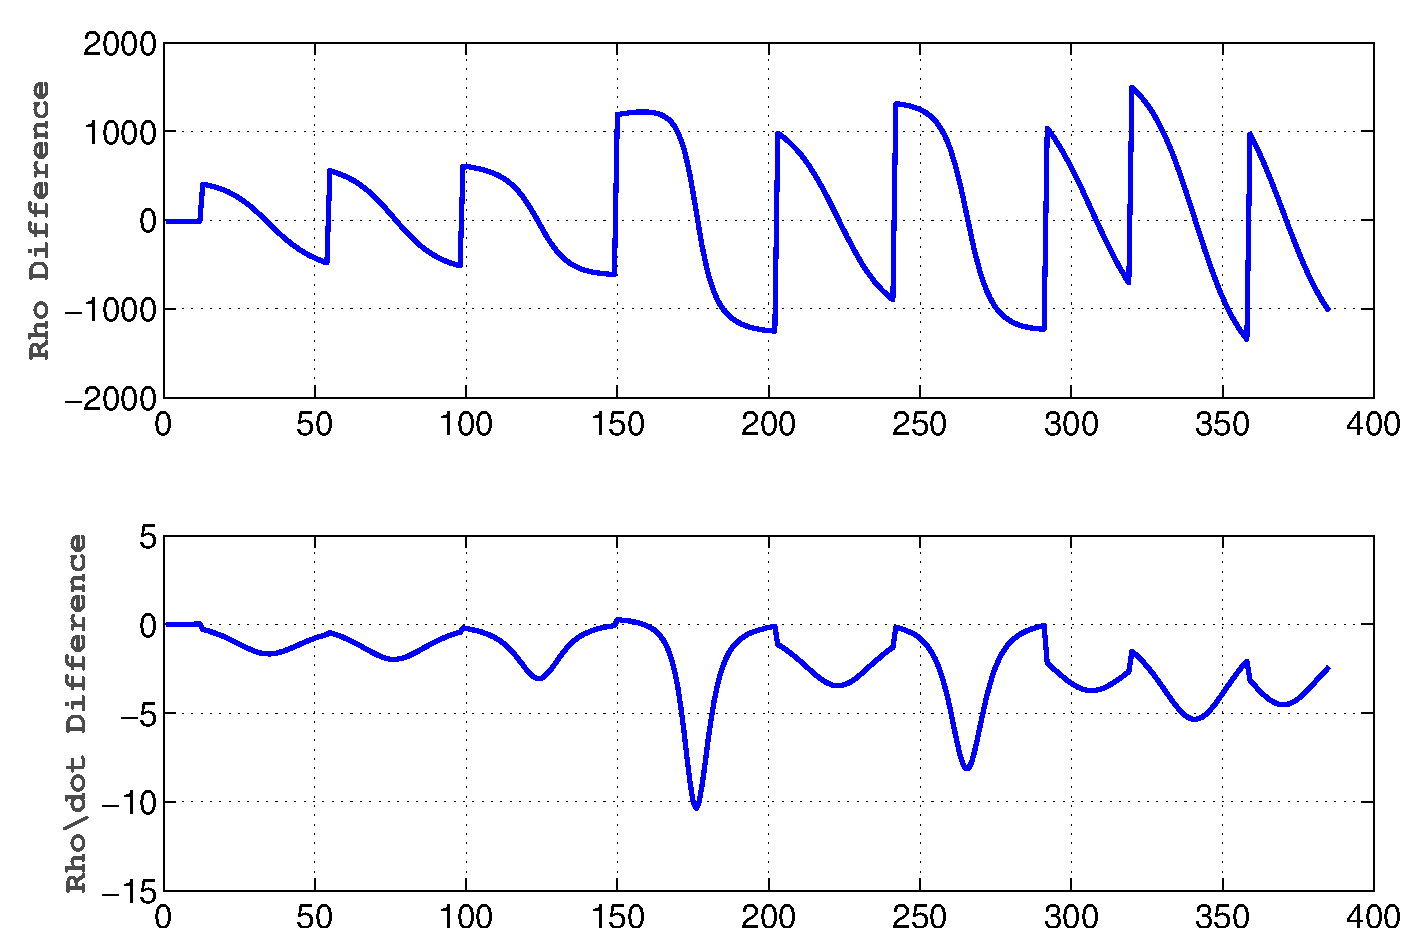
\includegraphics [width=4in]{HW7_main_01.eps}



\end{document}
    
